\FILE{section-workflow.tex}

\subsubsection{Analytics Service Pipelines}

\paragraph{Motivation.}
In many cases a big data analysis is split up in multiple
subtasks. These subtasks may be reusable in other analytics
pipelines. Hence it is desirable to be able to specify and use them in
a coordinated fashion allowing reuse of the logic represented by the
analysis. Users must have a clear understanding on what the analysis
is doing and how it can be invoked and integrated.

\paragraph{Access Requirements.}
The analysis must include a clear and easy to understand specification
that encourages reuse and provides sufficient details about its
functionality, data dependency and performance. Analytics services may
have authentication, autorotation and access controls build in that
enable access buy users controlled by the service providers.




\begin{figure}[htb]
\centering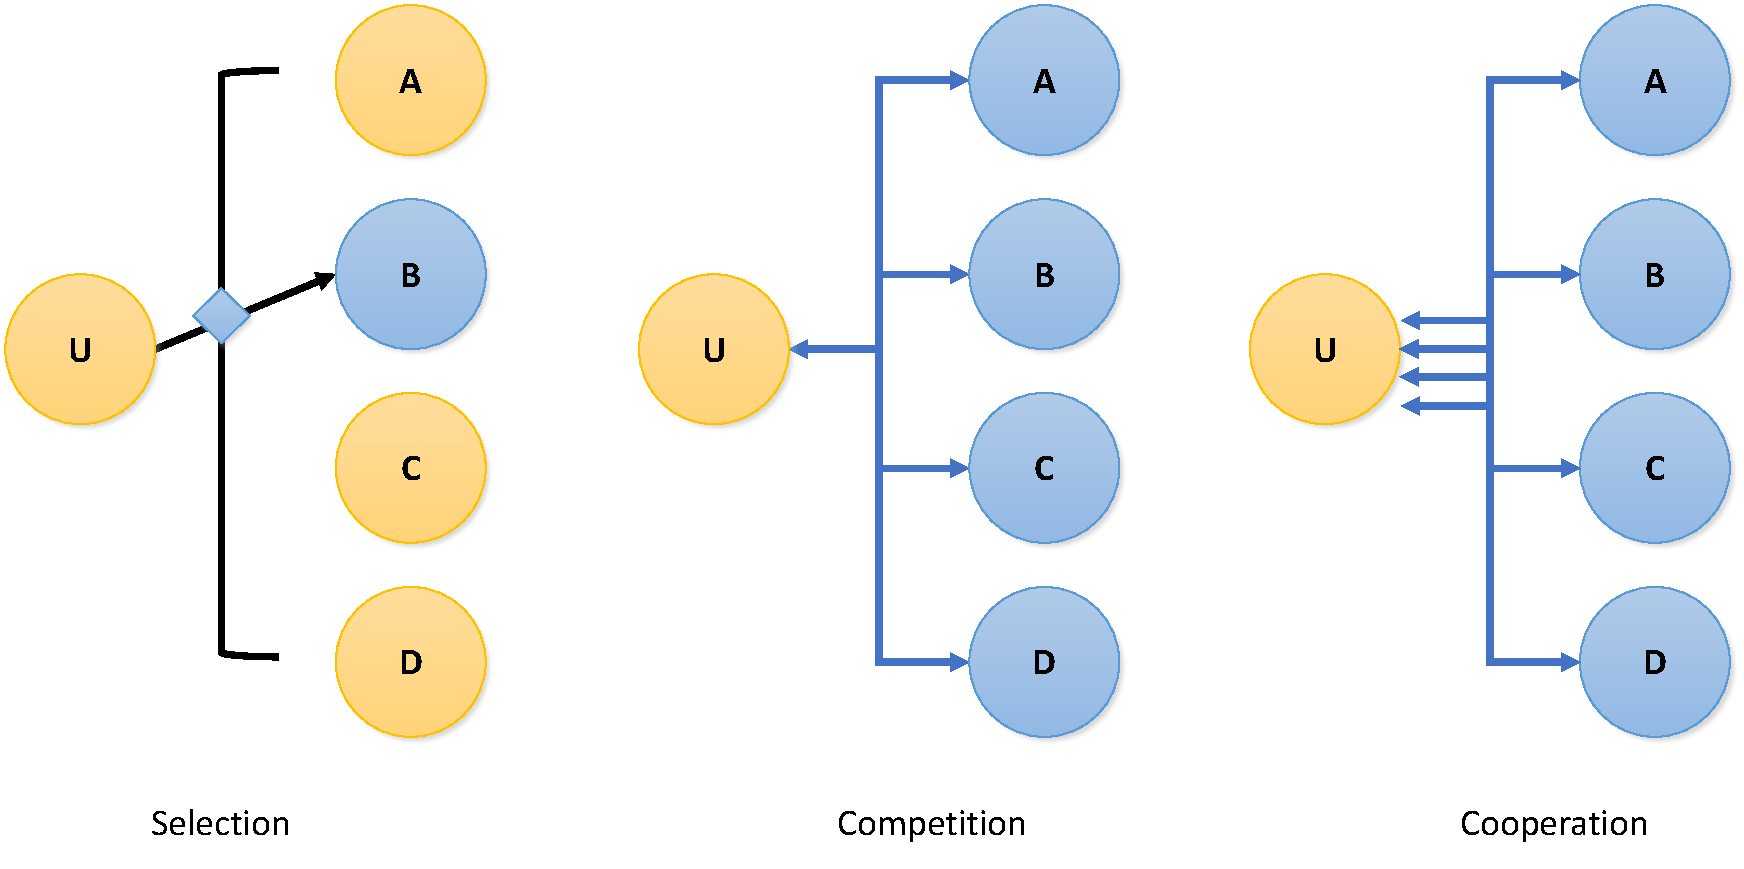
\includegraphics[width=1.0\columnwidth]{images/NIST-AI-services-workflow.pdf}
\label{fig:hvac-2}
\caption{Hybrid service integration.}
\end{figure}


\subsubsection{Federated Analytics Service Catalogue}
\subsubsection{Catalogue Attributes}
\subsubsection{Federated analytics service Registries}
\subsubsection{Registry Attributes}

\subsection{Resource Accessibility}
\subsubsection{Resource Management}
\subsubsection{Security}

